\section{Proposed Optimizations}
\label{sec:optimizations}

\subsection{Shared Memory problem}
\label{smp}
Shared memory is memory that can be used to pass data between cores, or to other applications. As the applications or cores can access the data just as any other data in the Random Access Memory (RAM) it is a very fast way of passing data between the applications, compared to regular message passing or software implementations such as UNIX domain sockets or CORBA. But it is less powerful, as all the processes has to run on the same machine.\cite{shared_memory}

At the moment TRAMP is using shared memory for inter-process communication (IPC). It allocates 32mb of memory, but the problem we have found is that we get a lot of packetloss due to the producer being faster than the consumers. This problem occurs when we are trying to send a file over the platform. The problem with the file sending is of course that the platform tries to send it as quickly as possible, where usual real-time applications such as skype sends a video stream that is not the total bandwidth, but 400kbps-1mbps (voice streams will be lower than this). When we try to limit the bandwidth on the producer we loose less packets.

Another thing about shared memory is that it is unsafe to use. The shared memory is accessible by all applications with user level access rights. This means that if a person has malware that wants to tamper with the data going over the shared memory there is no security to stop it. In a real-time application this might not be an issue, but for specific uses where security is important it is not recommended to use shared memory unless you encrypt the data in the producer.

\subsection{Data transfer rate}
As mentioned in section \ref{smp} we had a lot of packetloss due to the producer being faster than the consumers. This is because the main use for this framework is to make real-time applications mobile. While a file sharing system takes all available bandwidth. A real-time application usually does not take this amount of bandwidth and is therefore more resistant to the problems we are seeing in our implementation.

If the framework were to support file sharing we would have to add a control structure that would have the ability to tell the producer that the client cannot handle this amount of packets, a way to tell the producer that the client can handle more and a way to ask for a re transmit of a specific packet.

\subsection{Network topology}
\label{nettop}
When deciding on a network topology we need to know the scope and how we want the network to scale. If we want people to be able to talk with single persons inside the network we need a protocol like the skype protocol (see section \ref{skype}.

After looking into the TRAMP network topology we decided that what was partially implemented was a mesh-push network. We also noticed that the node chose one neighbor node that was the closest relative to the delay and subscribe to that node. This makes the node responsible for pushing all the packets he get from the specific label to the new node. We've also noticed that this does not work exactly as planned, 

\begin{center}
 \begin{figure}[h!]
  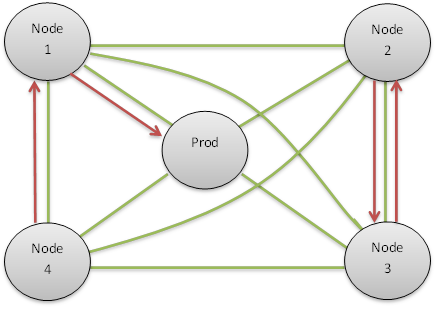
\includegraphics[width=250pt]{TrampNetworkTopology.png}
  \caption{TRAMP Network Topology}
  % TrampNetworkTopology.png: 436x309 pixel, 96dpi, 11.54x8.18 cm, bb=0 0 327 232
  \label{tramp_topology}
 \end{figure}
\end{center}

As we can see on figure \ref{tramp_topology} every node in the network connect to all the other nodes (the green lines), each node then chooses a ``closest neighbor to subscribe to (the red arrows). As you can see on the figure node 2 chooses node 3 and node 3 chooses node 2, this makes these nodes not in reach of the source node (the producer). This is one big fault with the topology we found.

To optimize the topology we recommend reading about the SopCast architecture (see section \ref{sopcast}). The differences we've found is that the TRAMP topology push the data to neighbor nodes, while the SopCast topology pull. This means that the nodes in the SopCast topology needs a bigger buffer in order to share with their neighbors. This will also fix the problem where the data inside the shared memory is overwritten before anyone can read it. SopCast also share all meta information in a tracker to minimize the strain on the network.

\subsection{UDP vs TCP}
User Datagram Protocol (UDP) was designed by David P- Reed in 1980, and defined in RFC768. UDP allows computer applications to send messages, or datagrams, to other hosts on an Internet Protocol(IP) without a setup phase like in Transmission Control Protocol(TCP). This stateless nature is also good for servers answering small queries from many clients. UDP also support packet broadcast (sending packets to all hosts on a local network) and multicasting (subscriber based).

UDP does not guarantee that the packet you sent ends up at the host. Neither does it support packet ordering (that packets reach the receiver in the correct order). This is what TCP is for. TCP was specified in RFC675 in December 1974. This protocol uses a three-way handshake in order to set up a connection between two hosts. It also provides reliable transmission, error detection, flow control and congestion control. 

\subsubsection{Real-time Transport Protocol}
The Real-time Transport Protocol (RTP) is a protocol developed by the Audio-Video Transport Working Group for the Internet Engineering Task Force (IETF). The first published RFC was published in 1996 with the code RFC1889. This was made obsolete by the newer RFC3550, published in 2003\cite{RFC3550}. This protocol is built on top of UDP and therefore does not provide Quality of Service (QoS) guarantees like delivery or packet order. The RPT standard defines two protocols. RTP and RTP Control Protocol (RTCP). This protocol provides QoS to the RTP protocol.

``RTP provides end-to-end network transport functions suitable for applications transmitting real-time data, such as audio, video or simulation data, over multicast or unicast network services.``\cite{RFC3550}

Due to the real-time nature of this protocol the majority of RTP implementations is build on UDP, but there are some implementations using TCP.





%shared mem problem
%sending data to fast (receiving too slow)

%delay(?)

%udp vs tcp or both